% Options for packages loaded elsewhere
\PassOptionsToPackage{unicode}{hyperref}
\PassOptionsToPackage{hyphens}{url}
%
\documentclass[
]{article}
\usepackage{lmodern}
\usepackage{amssymb,amsmath}
\usepackage{ifxetex,ifluatex}
\ifnum 0\ifxetex 1\fi\ifluatex 1\fi=0 % if pdftex
  \usepackage[T1]{fontenc}
  \usepackage[utf8]{inputenc}
  \usepackage{textcomp} % provide euro and other symbols
\else % if luatex or xetex
  \usepackage{unicode-math}
  \defaultfontfeatures{Scale=MatchLowercase}
  \defaultfontfeatures[\rmfamily]{Ligatures=TeX,Scale=1}
\fi
% Use upquote if available, for straight quotes in verbatim environments
\IfFileExists{upquote.sty}{\usepackage{upquote}}{}
\IfFileExists{microtype.sty}{% use microtype if available
  \usepackage[]{microtype}
  \UseMicrotypeSet[protrusion]{basicmath} % disable protrusion for tt fonts
}{}
\makeatletter
\@ifundefined{KOMAClassName}{% if non-KOMA class
  \IfFileExists{parskip.sty}{%
    \usepackage{parskip}
  }{% else
    \setlength{\parindent}{0pt}
    \setlength{\parskip}{6pt plus 2pt minus 1pt}}
}{% if KOMA class
  \KOMAoptions{parskip=half}}
\makeatother
\usepackage{xcolor}
\IfFileExists{xurl.sty}{\usepackage{xurl}}{} % add URL line breaks if available
\IfFileExists{bookmark.sty}{\usepackage{bookmark}}{\usepackage{hyperref}}
\hypersetup{
  hidelinks,
  pdfcreator={LaTeX via pandoc}}
\urlstyle{same} % disable monospaced font for URLs
\usepackage[margin=1in]{geometry}
\usepackage{graphicx}
\makeatletter
\def\maxwidth{\ifdim\Gin@nat@width>\linewidth\linewidth\else\Gin@nat@width\fi}
\def\maxheight{\ifdim\Gin@nat@height>\textheight\textheight\else\Gin@nat@height\fi}
\makeatother
% Scale images if necessary, so that they will not overflow the page
% margins by default, and it is still possible to overwrite the defaults
% using explicit options in \includegraphics[width, height, ...]{}
\setkeys{Gin}{width=\maxwidth,height=\maxheight,keepaspectratio}
% Set default figure placement to htbp
\makeatletter
\def\fps@figure{htbp}
\makeatother
\setlength{\emergencystretch}{3em} % prevent overfull lines
\providecommand{\tightlist}{%
  \setlength{\itemsep}{0pt}\setlength{\parskip}{0pt}}
\setcounter{secnumdepth}{-\maxdimen} % remove section numbering
\usepackage{bm}
\usepackage{booktabs}
\usepackage{longtable}
\usepackage{array}
\usepackage{multirow}
\usepackage{wrapfig}
\usepackage{float}
\usepackage{colortbl}
\usepackage{pdflscape}
\usepackage{tabu}
\usepackage{threeparttable}
\usepackage{threeparttablex}
\usepackage[normalem]{ulem}
\usepackage{makecell}
\usepackage{xcolor}

\author{}
\date{\vspace{-2.5em}}

\begin{document}

\hypertarget{methods}{%
\subsection{Methods}\label{methods}}

We want to estimate the probability that an encrypted vote \(V\) with
byte length \(B\) is for candidate \(k\), \(\pi(V_k \vert B)\). Bayes'
rule allows us to rewrite this probability as

\[ \pi(V_k \vert B) = \dfrac{\pi(B \vert V_k) \pi (V_k)}{ \pi(B)} \>. \]

\noindent Here, \(\pi(V_k)\) is known as \textit{the prior} and is
interpreted as the proportion of people expected to vote for candidate
\(k\) prior to the election. The quantity \(\pi(B \vert V_k )\) is known
as \textit{the likelihood} and can be interpreted as the probability of
observing an encrypted vote of byte length \(B\) for candidate \(k\).
The denominator \(\pi(B)\) is a normalizing constant and can be ignored
for our purposes, meaning
\(\pi(V_k \vert B) \propto \pi(B\vert V_k)\pi(V_k)\).

To classify which candidate the encrypted vote is for given a byte
length, we choose the candidate \(k\) who maximizes the posterior
probability

\begin{align*}
\widehat{V}_k &= \underset{k \in K}{\arg\max} \left\{  \pi(V_k \vert B)  \right\} \>, \\
& = \underset{k \in K}{\arg\max} \left\{  \pi(B\vert V_k)\pi(V_k)  \right\} \>.
\end{align*}

\noindent Generally, \(\pi(B\vert V_k)\) is unknown. However,
simplifying assumptions can be used to facilitate prediction. In
particular, if we consider byte length as a categorical variable then we
can assume the likelihood for byte length is multinomial

\[ \pi(B \vert V_k) = \operatorname{Multinomial}(\bm{\theta}_k) \>. \]

\noindent Here, the multinomial parameter \(\bm{\theta}_k\) is indexed
by \(k\) to allow for different candidates to have different
probabilities for observing various byte lengths. Making this assumption
on the likelihood leads to the \textit{Multinomial Naive Bayes Model}.
Using data with labelled votes and byte lengths, the \(\bm{\theta}_k\)
can be estimated and then used to make predictions.

In what follows, we fit a Multinomial Naive Bayes Model and evaluate
it's out of sample performance on predicting which candidate a vote is
for given the encrypted vote's byte length.

\hypertarget{model-evaluation}{%
\subsection{Model Evaluation}\label{model-evaluation}}

We perform 100 repeats of 10 fold cross validation to evaluate our
model. Briefly, \(v\)-fold cross validation is a technique to estimate
out of sample performance of a predictive model. Data are split into
\(v\) equally sized and disjoint subsets (in our case, \(v=10\)). To
estimate the out of sample performance, \(v-1\) subsets are combined and
used to fit the model. The model is then used to predict on the
remaining subset of data. Performance metrics are calculated on these
predictions. This process is repeated until all \(v\) subsets have acted
as a hold out set. The performance metrics are averaged over the \(v\)
subsets. Repeating \(v\) fold cross validation 100 times is a way of
avoiding spurious performance estimates based on fortuitous splits.

We evaluate model classification ability using three metrics: accuracy,
precision, recall. Interpretation of each metric is as follows:

\begin{description}
\item[Accuracy] is the proportion of correctly identified votes.  Probabilistically, accuracy is the probability the vote is correctly identified, $\pi(\widehat{V}_k = V_k)$.

\item[Precision] is the proportion of predictions for candidate $k$ which correctly identify a vote for candidate $k$.  Probabilistically, the precision is the probability the vote is for candidate $k$ conditioned on the prediction being for candidate $k$, $\pi(V_k \vert \widehat{V}_k)$.  As an example, suppose in our sample we predict 100 votes will be for candidate $k$.  Of those 100, 72 are actually for candidate $k$.  The precision for candidate $k$ is then $0.72 = 72/100$.

\item[Recall] is the proportion of votes for candidate $k$ which are correctly predicted to be for candidate $k$.  Probabilistically, recall is the probability the prediction made is for candidate $k$ conditioned on the vote being for candidate $k$, $\pi(\widehat{V}_k \vert V_k)$.  As an example, suppose in our sample there are 100 votes for candidate $k$.  Of those 100 votes, we correctly predict that 78 votes will be for candidate $k$.  The recall is then $0.78=78/100$.        
\end{description}

We report the average accuracy, precision, and recall over the 100
repeats of 10 fold cross validation as well as 2 standard deviations.

\newpage

\hypertarget{experiment-1}{%
\subsection{Experiment 1}\label{experiment-1}}

\begin{figure}[h!]

{\centering 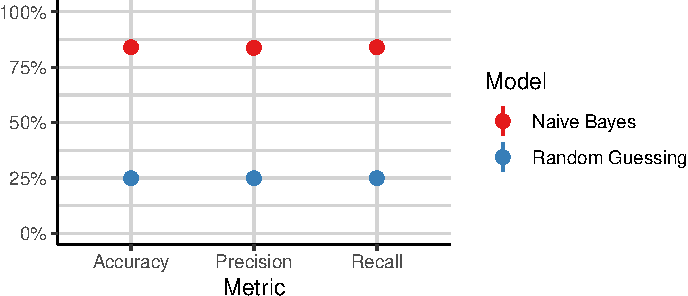
\includegraphics{Untitled_files/figure-latex/experiment-1-1} 

}

\caption{Comparison of a Naive Bayes model (red) and a hypothesized "best" strategy of random guessing (blue).  The ballot in this example has 4 candidates, meaning that the best accuracy that could be achieved -- at least in theory -- is 25\%. The Naive Bayes model has a cross validated accuracy, precision, and recall of nearly 84\%, meaning 84 of every 100 votes are correctly classified using byte length alone.  Class specific accuracy varies among candidates, with some candidates seeing very high accuracy (~90\%) while others see smaller accuracy (~60\%).  However, accuracy across all classes is consistently larger than the expected 25\%.}\label{fig:experiment-1}
\end{figure}

\hypertarget{experiment-2}{%
\subsection{Experiment 2}\label{experiment-2}}

\begin{center}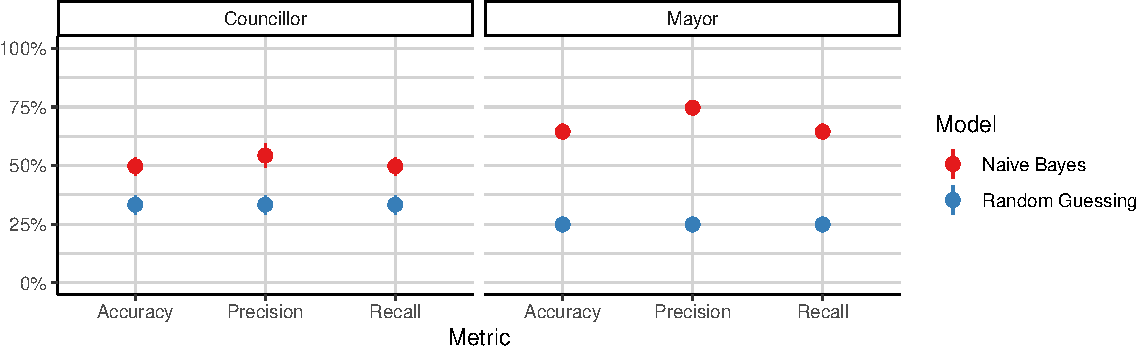
\includegraphics{Untitled_files/figure-latex/experiment-2-1} \end{center}

\hypertarget{experiment-3}{%
\section{Experiment 3}\label{experiment-3}}

\begin{center}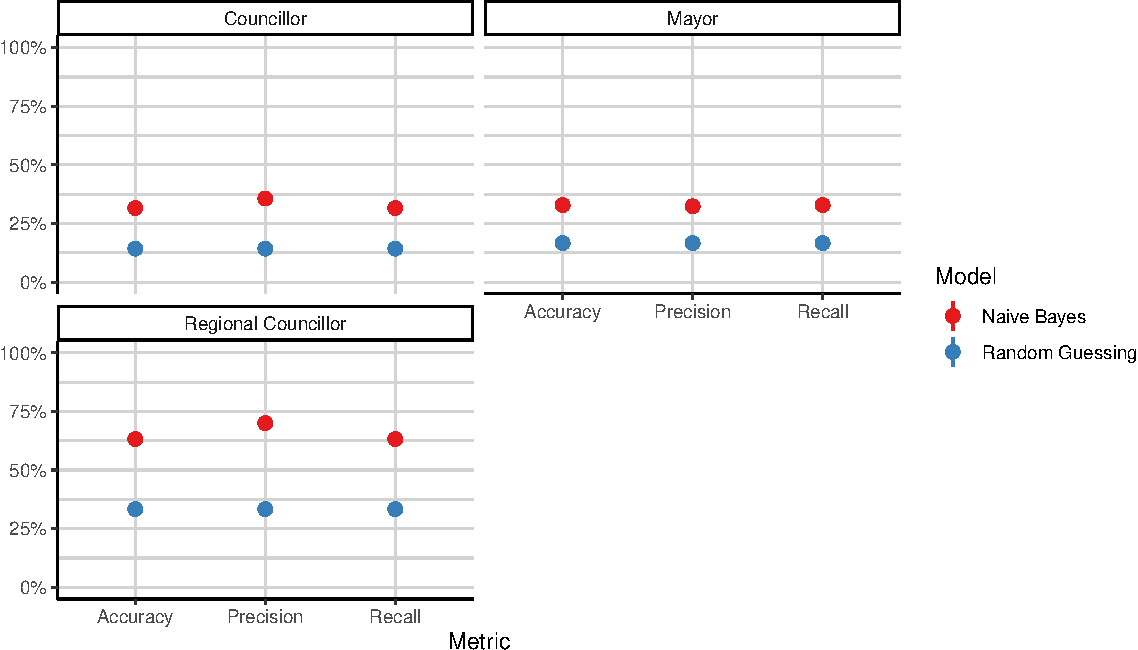
\includegraphics{Untitled_files/figure-latex/unnamed-chunk-1-1} \end{center}

\hypertarget{conclusion}{%
\subsection{Conclusion}\label{conclusion}}

Generally, we find our models do better than the assumed baseline of
random guessing. The performance varies depending the ballot structure,
but we are able to achieve an accuracy between 14 and 60 percentage
points higher than what should be achievable under the assumption that
votes are completely hidden and no information can be used to identify
votes. Validation of our models shows that this difference in
performance is very unlikely to be explained by sampling variation, and
could be considered statistically significant, although we don't perform
any statistical tests to that affect.

\end{document}
